\qt{Spouses, Part I\label{husbands_wives_correlation}}
The Great Britain Office of Population Census and Surveys once 
collected data on a random sample of 170 married women in 
Britain, recording the age (in years) and heights (converted 
here to inches) of the women and their spouses.\footfullcite{Hand:1994} 
The scatterplot on the left shows the spouse's age plotted against the woman's age, and the plot on the right shows spouse's height 
plotted against the woman's height.
\begin{center}
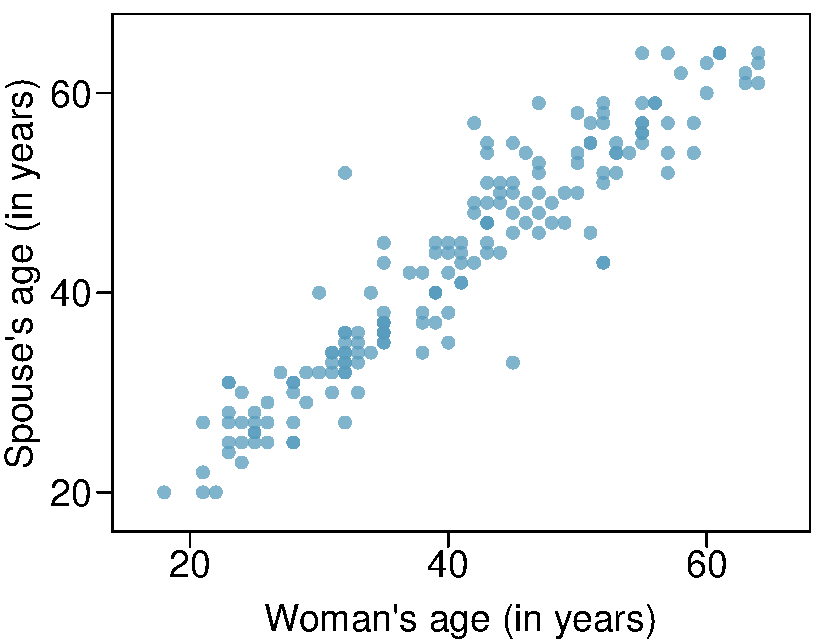
\includegraphics[width=0.36\textwidth]{figures/husbands_wives_age} 
\hspace{5mm}
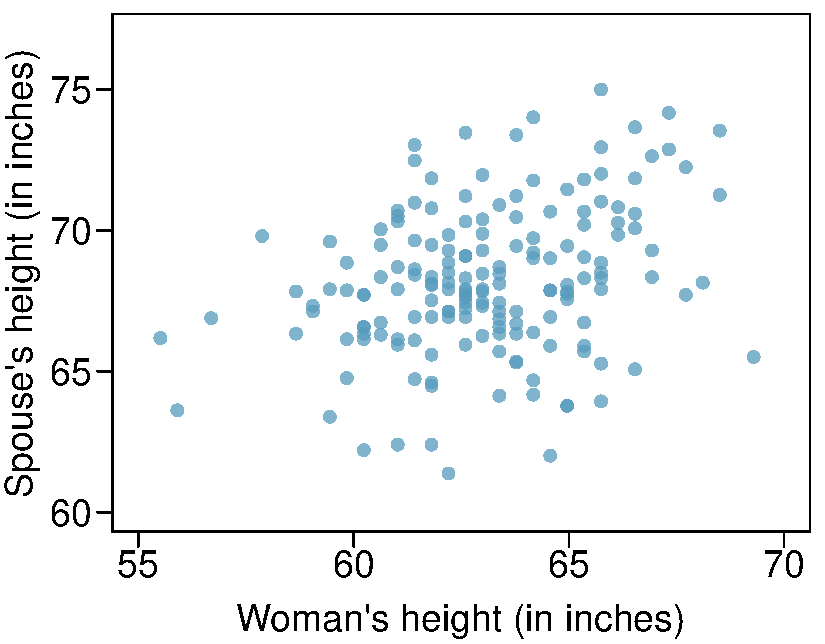
\includegraphics[width=0.36\textwidth]{figures/husbands_wives_height}
\end{center}
\begin{parts}
\item Describe the relationship between the ages of women in the sample and their spouses' ages.
\item Describe the relationship between the heights of women in the sample and their spouses' heights.
\item Which plot shows a stronger correlation? Explain your reasoning.
\item Data on heights were originally collected in centimeters, and 
then converted to inches. Does this conversion affect the correlation 
between heights of women in the sample and their spouses' heights?
\end{parts}